\documentclass[a4paper,10pt]{article}
\usepackage[utf8]{inputenc}
\usepackage{graphicx}
\usepackage{hyperref}
\usepackage{minted}
%opening
\title{The Memory \& Storage Design of Neo4J}
\author{Fabian Klopfer}

\begin{document}

\maketitle

\begin{abstract}
In this document I describe the internals of the storage layer of the popular native graph database Neo4J. A detailed description of how records are stored into which files and how these are accessed is to be elaborated on in the following article. This is a translation, update and extension of previous work done by Michael Brendle. 
\end{abstract}



\section{Introduction}
Relational databases store tables of data. The links considered in this category of DBMS are mostly used to stitch together the fields of an entry into one row again, after it has been split to satisfy a certain normal form. Of course one may also store tables where one table stores nodes and the other table's fields are node IDs to represent relationships.

However, in order to traverse the graph, one has either to do a lot of rather expensive look ups or store auxiliary structures to speed up the look up process. In particular when using B-trees as index structure, each look up takes $\mathcal{O}(\log(n))$ steps to locate a specific edge. Alternatively one could store an additional table that holds edge lists such that the look up of outgoing or incomming edges is only $\mathcal{O}(\log(n))$ which would speed up breadth first traversals. But still one has to compute joins in order to continue the traversal in terms of depth. Another way to speed things up is to use a hash-based index, but this also has a certain overhead aside from the joins.

In contrast to relational data base management systems, native graph databases use structures specialised for this kind of queries. In the remainder of the document I discuss based upon Michael Brendle's work what structures and mechanisms the graph database Neo4J uses in order to achieve this superior performance in the domain of graphs.

First of all, let us consider the high level architecture of a database management systems - with a focus on the storage and loading elements.

\begin{figure}[htp]
 \begin{center}
  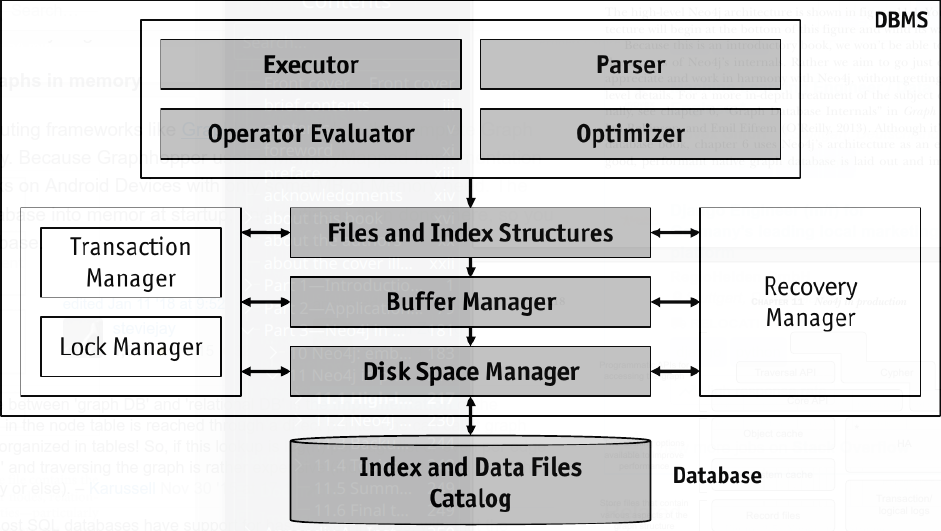
\includegraphics[keepaspectratio,width=\textwidth]{img/RDBMS.png}
 \end{center}
 \caption{The typical structure of a relational database management system } %TODO citation
\end{figure}
Here The disk space manager, sometimes also called storage manager, handles de-/allocations, reads \& writes and provides the concept of a page: A disk block brought into memory. For that it needs to keep track of free blocks in the allocated file. Optimally both a disk block and a page are of the same size. One crucial task of a disk space manager is to store sequences of pages into continuous memory blocks in order to optimize data locality. Data locality has the upside, that one needs only one I/O operation to load multiple pages. To summarize the two most important objectives of a storage manager are to provide a locality-preserving mapping from pages to blocks based upon the information in the DBMS and to abstract physical storage to pages, taking care of allocation and access.
A buffer manager is used to mediate between external storage and main memory. It maintains a designated pre-allocated area of main memory --- called the buffer pool --- to load, cache and evict pages into or from main memory. It's objective is to minimize the number of disk reads to be executed by caching, pre-fetching and the usage of suitable replacement policies. It also needs to take care of allocating a certain fraction of pages to each transaction.
The final memory and storage model relevant component of the  of a database management system is the file layout and possible index structures. 
% FIXME continue here with michaels slides 01-74
% TODO add high-level overview of N4J (emil and fusion of older ones)

\section{Disk Space Management or Storage Management}
\mintinline{bash}{
neo4j/community/io/src/main/java/org/neo4j/io/fs/
} \\

\mintinline{bash}{neo4j/community/storage-engine-api/src/main/java/org/neo4j/storageengine/api/} \\

\mintinline{bash}{neo4j/community/native/src/main/java/org/neo4j/internal/nativeimpl/LinuxNativeAccess.java} \\

\href{Hpw delete works}{https://neo4j.com/developer/kb/how-deletes-workin-neo4j/} \\

\href{G-Store}{http://g-store.sourceforge.net/th/index.htm} \\

\href{Algorithms \& data structures}{https://www.youtube.com/watch?v=NlT21Ceg3y0}  \\

\href{Reusing space}{https://neo4j.com/docs/operations-manual/current/performance/space-reuse/\#space-reuse} \\


\section{Buffer Management}
% TODO use michael brendles work
\mintinline{bash}{
neo4j/community/io/src/main/java/org/neo4j/io/pagecache
}

\href{Page Cache layout ??? Outdated ???}{https://www.slideshare.net/thobe/an-overview-of-neo4j-internals} \\


\section{File Layout, Record Structure \& Management}
\mintinline{bash}{neo4j/community/record-storage-engine/.../kernel/impl/store/record/}

\mintinline{bash}{neo4j/community/record-storage-engine/src/main/java/org/neo4j/kernel/impl/store/} \\

\href{Layout N4J}{https://neo4j.com/developer/kb/understanding-data-on-disk/} \\

Ancient: \href{Slides: Internals Of N4J}{https://www.slideshare.net/thobe/an-overview-of-neo4j-internals} \\
\href{Video}{https://skillsmatter.com/skillscasts/2968-neo4j-internals} \\

\href{N4J Arch blog}{http://key-value-stories.blogspot.com/2015/02/neo4j-architecture.html} \\

\href{Followup discussion w devs}{https://groups.google.com/g/neo4j/c/cxClivwF94k}

\section{Example}
% TODO adapt from Brendle

\section{Conclusion}

\end{document}
